\subsection*{Blobs}\label{sec:blobs}
En blob er en sammenhængende region af pixels, der enten er betydeligt lysere eller mørkere end dens omgivelser, altså områder, der står i kontrast til deres baggrund. En blob kan derfor udvælges som værende et lokalt ekstrema i billedet.
I figur \ref{fig:lindblob1} ses tre lyse blobs, på en mørk baggrund, illustreret som bakketoppe. Der hvor bakkerne mødes, eksisterer et punkt, hvor dets hældning krummer op i en retning og krummer ned i en anden. Et sådant punkt kaldes et sadel-punkt. Et sadel-punkt er ikke et ekstrema, og derfor ikke en blob.
\begin{figure}[H]
    \centering
    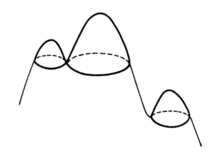
\includegraphics[width=0.35\textwidth]{fig/44.png}
    \vspace{-0.5em}   
    \begin{center}
    \caption{{\footnotesize \textit{
    Tre lyse blobs på en mørk baggrund illustreret i 2 dimensioner \cite{blob}}}}
    \label{fig:lindblob1}
     \end{center}
  \end{figure}
       \vspace{-2.7em}
\noindent
En blob kan udvælges ved at identificere den geometriske struktur i om omkring et punkt. De to principale krumninger i et punkt angiver, hvor meget overfladen bøjer i de forskellige retninger. Da et ekstrema angiver en blob, vil fortegnet for de to principale krumninger være ens. For et punkt placeret på et maksima vil de principale krumninger være konkave (nedadgående) og for et punkt placeret på et minima vil de principielle krumninger være konvekse (opadgående). For et punkt placeret på et sadel-punkt, vil den ene krumning være konkav og den anden konveks. \\ 
Om et punkt i billedet er placeret på et maksima, minima eller sadel-punkt, kan bestemmes ved en 'to variabel, anden-afledte-test'. Dette udføres ved at opstille en matrice, for et givent punkt, der indeholder dens dobbeltafledte i $x, y \text{ og } xy$ retningen også kaldet Hessian matricen $\mathcal{H}$.
\begin{equation}
\mathcal{H} = 
 \begin{bmatrix}
 	L_{xx} & L_{xy} \\
 	L_{xy} & L_{yy}
 \end{bmatrix}
 \label{hessianmatrixblob}
\end{equation}
hvor den andenafledte i $x$ retningen defineres ved:
\begin{equation}
L_{xx}(x,y,\sigma) = (\frac{\partial^2 }{\partial x^2 } G(x,y,\sigma)) * I
\label{lxx}
\end{equation}
Egenvektorerne for Hessian matricen beskriver retningerne af de principale krumninger af et punkt, hvor egenværdierne beskriver størrelserne af disse krumninger. Hessian matricens egenværdier $\lambda_1,\lambda_2$, kan bruges til at lokalisere blobs.
\begin{equation}
\begin{split}
indikator = 
\begin{cases}
\text{Minima} & \text{hvis } \lambda_1, \lambda_2 > 0, \\
\text{Maksima}& \text{hvis } \lambda_1, \lambda_2 < 0,  \\
\text{Sadel-Punkt} & \text{hvis } \lambda_1 \lambda_2 < 0.
\end{cases}
\end{split}
\label{maxsurp}
\end{equation}
Egenværdiernes fortegn kan estimeres ved  at finde determinanten af Hessian matricen:
\begin{equation}
\textbf{det}\mathcal{H} = L_{xx}L_{yy}-L_{xy}^2
\label{detofhessian}
\end{equation}
Da $\bold{det}(\mathcal{H})=\lambda_1 \lambda_2$, vil fortegnet af determinanten angive om et punkt er et ekstrema eller et sadel-punkt. Figur \ref{fig:makssad} illustrere, hvordan Hessian matricen approksimere den geometriske struktur i billedet med et andengradspolynomium. Figuren viser approksimeringen, med et punkt lokaliseret på et maksima og et sadel-punkt.
\begin{figure}[H]
    \centering
    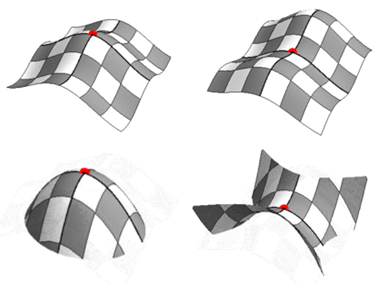
\includegraphics[width=0.50\textwidth]{fig/41.png}
    \vspace{-0.5em}
    \begin{center}
    \caption{{\footnotesize \textit{Venstre: Et punkt placeret på et makisma. Højre: Et punkt placeret på et sadel-punkt. Nedestående tilsvarende figurer, viser hvordan hessian matricen approksimere billedet, med et andengradspolynomium. 
}}}
    \label{fig:makssad}
     \end{center}
  \end{figure}
       \vspace{-2.7em}
\noindent
En anden metode at detektere blobs er ved Laplace operatoren, som giver et stærkt filtersvar i centeret af en blob. Laplace operatoren kan defineres ved:
\begin{equation}
\nabla^2L(x,y) = L_{xx}+L_{yy}
\end{equation}
Da Laplace operatoren svarer til sporret af Hessian matricen $\bold{Tr}(\mathcal{H}) = \lambda_1 + \lambda_2$, vil filtersvaret fra Laplace operatoren $\nabla^2L$ fortælle noget om egenværdierne. Et stort negativt filtersvar, vil angive et maksima, da egenværdierne begge vil være negative. Et stort positivt filtersvar vil angive et minima, da egenværdierne begge vil være positive. Et stort filtersvar vil dog ikke altid angive et ekstrema, og derfor ikke en blob. En egenværdi med en stor absolut værdi og den anden med en lille værdi vil angive en kant, men stadig resultere i et stort filtersvar.
\label{laplaceblob}
%\end{equation}
Anvendes Laplace operatoren på Gaussfunktionen (opskrevet i ligning \eqref{2dgaussian}), kan resultatet diskretiseres og anvendes som en kerne, der kan foldes med et billede for identifere forekomster af blobs.
\begin{equation}
LoG= \nabla^2 G
\label{lap}
\end{equation}
Som nævnt vil et stort filtersvar (postivit eller negativt) til Laplace Gauss filteret definere en blob. Dette er dog kun tilfældet, hvis størrelsen af Laplace Gauss filteret, svarer til størrelsen af blobben. En tilgang til dette er systematisk at forøge størrelsen af Laplace Gauss filteret, for det eksisterende skalarum, og udvælge skalaen, hvor der afgives et maksimalt filtersvar. Figur \ref{fig:laprespons} illustrere et filtersvar for en blob, der er foldet, med et et Laplace Gauss filter af stigende sigmaværdi. Det ses at når blobben er betydeligt større end sigmaværdien af filteret, vil filtrersvaret være småt. Når sigmaværdien på filteret forøges, afgives et stort filtersvar. Når sigmværdien forøges yderligere, flades filtersvaret ud, som set i nederste billede i figur \ref{fig:laprespons}. Næstsidste billede viser en sigmastørrelse, der giver et maksimalt filtersvar til blobstørrelsen.
\begin{figure}[H]
    \centering
    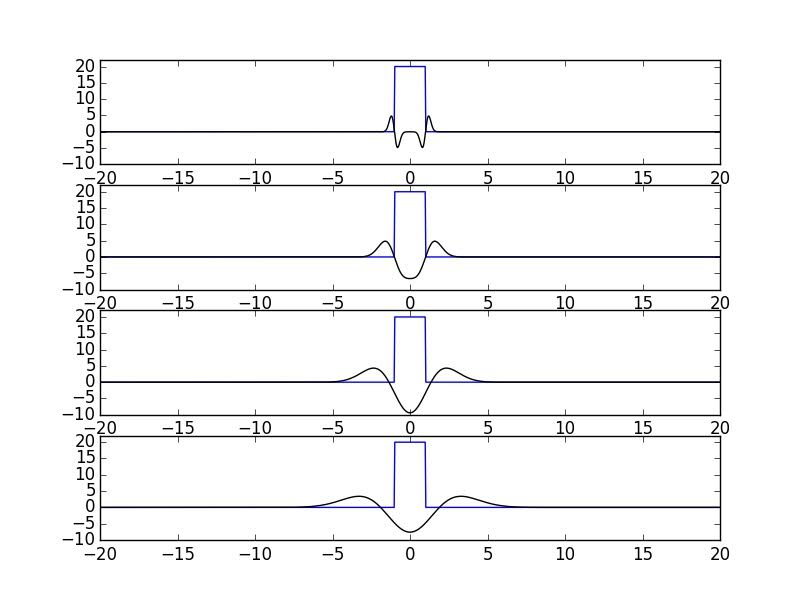
\includegraphics[width=0.80\textwidth]{fig/42.jpg}
    \vspace{-0.75em}
    \begin{center}
    \caption{{\footnotesize \textit{En blob (den lysseblå firkant) udsat for et skalanormaliseret Laplace Gauss filter af stigende sigmaværdi, hvor filtersvaret er illustreret ved en sort streg.
}}}
    \label{fig:laprespons}
     \end{center}
  \end{figure}
       \vspace{-2.7em}
\noindent
En egenskab ved skalarums-repræsentationen er at amplituden af de rumlige afledte vil falde. Dette er, som nævnt i afsnit \ref{sec:scale}, grundet at maksima over skala ikke vil forøges og at minima ikke formindskes. Amplituden af ekstremaer vil derfor altid formindskes over skala \cite{phdlind}. Dette resulterer i at filtersvaret for $LoG$, vil formindskes når skalaparametren øges. For at muliggøre en sammenligning af filtersvaret over skala, normaliseres filtersvaret ift. skala.  Lindenberg \cite{lindenscale} viser at ved anvendelse af billedets afledte af orden $p$, skal skalanormalisering udføres ved at multiplicere filtersvaret med $\sigma^p$. Da $LoG$ anvender de andenafledte af et Gauss filter, multipliceres filtersvaret med $\sigma^2$. En skalanormaliseret Laplacian of Gauss, kan derfor opskrives som:
\begin{equation}
\sigma^2 \nabla^2G = \sigma^2(L_{xx}+L_{yy})
\end{equation}